\subsubsection{Graph Methods}
\label{sec:methods.structured.graph}

% Author: Flo

If data can be considered a graph-like structure, where two related features are
connected with an edge, it turns out to increase the performance of classifiers
to find connected components and accept/discard whole components at once
(\cite{Jacob:09}). 

\begin{figure}[!ht]
  \centering 
  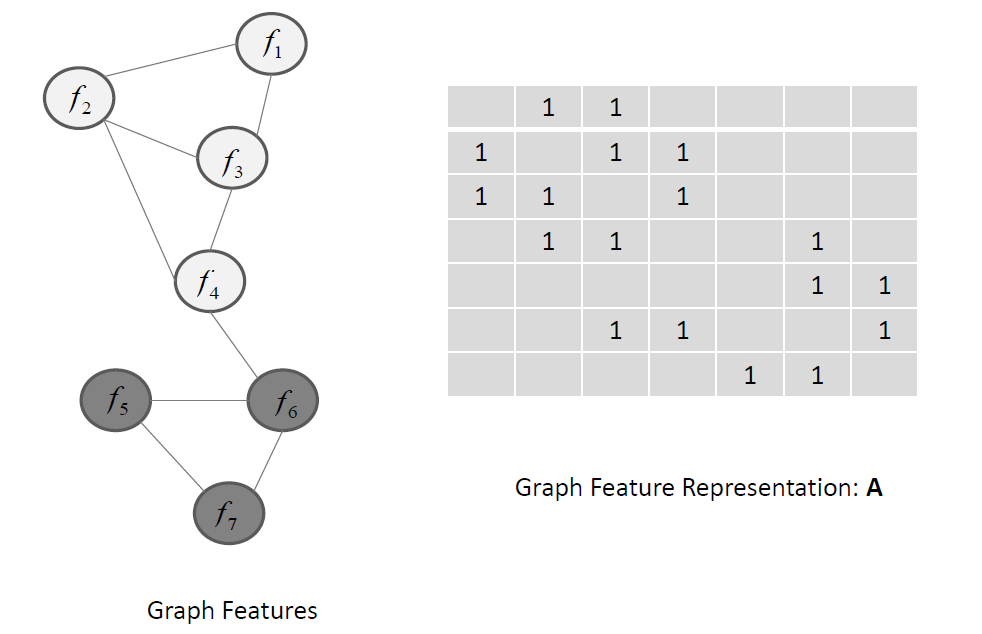
\includegraphics[width=0.8\textwidth]{chapters/methods/structured/graph_lasso}
  \caption{Reprinted from \cite{Tang:14}. Illustration of features forming a
  graph-structurem where $A$ is the adjacency-matrix (\cite{Tang:14}).}
  \label{fig:methods.structured.graph.lasso}
\end{figure}

Figure \ref{fig:methods.structured.graph.lasso} shows a
possible graph of $7$ features and its adjacency matrix. In this figure the
features $f_5$, $f_6$, $f_7$ are likely to be selected or discarded together.

The graph lasso method (\cite{Jacob:09}) can be used formulate an
energy-equation for the graph that needs to be minimized. Common
energy-minimization-techniques can then assign weights to parts of the graph,
which can be used to discard non-relevant features.
